\section{Конструкторский раздел}

\subsection{Общая структура решения}

Разрабатываемое решение включает два основных компонента:
\begin{itemize}
	\item загружаемый модуль ядра Linux, регистрирующий виртуальное устройство ввода типа «мышь» в подсистеме ввода и принимающий команды по RFCOMM-соединению Bluetooth~\cite{linux-input-docs,input-programming,bluetooth-core-spec,bluez-rfcomm-wiki};
	\item мобильное приложение для Android, устанавливающее RFCOMM-соединение с рабочей станцией и преобразующее действия пользователя на сенсорном экране в последовательность бинарных сообщений фиксированного формата~\cite{android-bt-connect,BluetoothSocket-doc}.
\end{itemize}

Модуль ядра взаимодействует с подсистемой ввода через структуру \lstinline|struct input_dev| и функции генерации событий ввода~\cite{linux-input-docs,input-programming}, а с подсистемой Bluetooth --- через серверный сокет с семейством \lstinline|PF_BLUETOOTH| и протоколом \lstinline|BTPROTO_RFCOMM|~\cite{bluetooth-core-spec,kernel-net-kapi,linux-rfcomm-core}. Мобильное приложение использует стек Bluetooth Android и API \lstinline|BluetoothAdapter|, \lstinline|BluetoothDevice| и \lstinline|BluetoothSocket| для установления соединения с модулем ядра и обмена бинарными сообщениями~\cite{android-bt-connect,BluetoothSocket-doc}.

\begin{figure}[h!]
	\centering
	\includegraphics[width=0.95\textwidth]{idef0.drawio.png}
	\caption{IDEF0-диаграмма подсистемы управления курсором с телефона}
	\label{fig:idef0}
\end{figure}
\clearpage

\subsection{Базовые структуры и точки входа драйвера}

Загружаемый модуль ядра использует следующие точки входа~\cite{linux-driver-basics}:
\begin{itemize}
	\item функцию инициализации, регистрируемую через макрос \lstinline|module_init|, выполняющую создание виртуального устройства ввода, настройку RFCOMM-сокета и запуск служебного потока;
	\item функцию завершения, регистрируемую через макрос \lstinline|module_exit|, выполняющую остановку служебного потока, закрытие RFCOMM-сокета и снятие виртуального устройства с регистрации в подсистеме ввода;
	\item функцию служебного потока обработки соединения, создаваемого с помощью \lstinline|kthread_run| и выполняющего цикл приёма команд по RFCOMM и генерацию событий ввода~\cite{linux-kthread-man}.
\end{itemize}

Для интеграции с подсистемой ввода используется структура \lstinline|struct input_dev|, в которой настраиваются:
\begin{itemize}
	\item поддерживаемые типы событий \lstinline|EV_REL| и \lstinline|EV_KEY|;
	\item коды событий \lstinline|REL_X|, \lstinline|REL_Y|, \lstinline|BTN_LEFT|, \lstinline|BTN_RIGHT|;
	\item идентификаторы производителя, продукта и человекочитаемое имя устройства~\cite{linux-input-docs,input-programming}.
\end{itemize}
Генерация событий выполняется вызовами \lstinline|input_report_rel|, \lstinline|input_report_key| и \lstinline|input_sync| для зарегистрированного устройства~\cite{linux-input-docs}.

Для взаимодействия с RFCOMM создаётся серверный Bluetooth-сокет с семейством \lstinline|PF_BLUETOOTH| и протоколом \lstinline|BTPROTO_RFCOMM|. Адрес сокета задаётся структурой адреса с полями семейства адресов, Bluetooth-адреса устройства и номера RFCOMM-канала, после чего выполняются операции привязки и перевода сокета в режим прослушивания~\cite{bluetooth-core-spec,kernel-net-kapi,linux-rfcomm-core}.

\subsection{Последовательность работы модуля ядра}

Работа модуля ядра логически разделяется на три этапа: инициализацию, обслуживание соединения и завершение работы.

На этапе инициализации выполняются проверка параметров, регистрация виртуального устройства ввода в подсистеме input, создание и настройка серверного RFCOMM-сокета и запуск служебного потока обработки соединения. Последовательность действий функции инициализации представлена на рис.~\ref{fig:module-load-scheme}.

\begin{figure}[h!]
	\centering
	\includegraphics[width=0.95\textwidth]{module_load_scheme.drawio.png}
	\caption{Схема алгоритма инициализации модуля ядра \texttt{phone\_mouse\_bt}}
	\label{fig:module-load-scheme}
\end{figure}
\clearpage

Служебный поток \lstinline|rx_loop| реализует цикл ожидания входящего RFCOMM-соединения, приёма и проверки сообщений фиксированной длины, обработки разрыва соединения и передачи декодированных команд во внутренние обработчики, генерирующие события ввода. Логика работы потока, включая обработку временного отсутствия данных, разрыва соединения и игнорирования некорректных пакетов, показана на рис.~\ref{fig:rx-loop-scheme}.
\begin{figure}[h!]
	\centering
	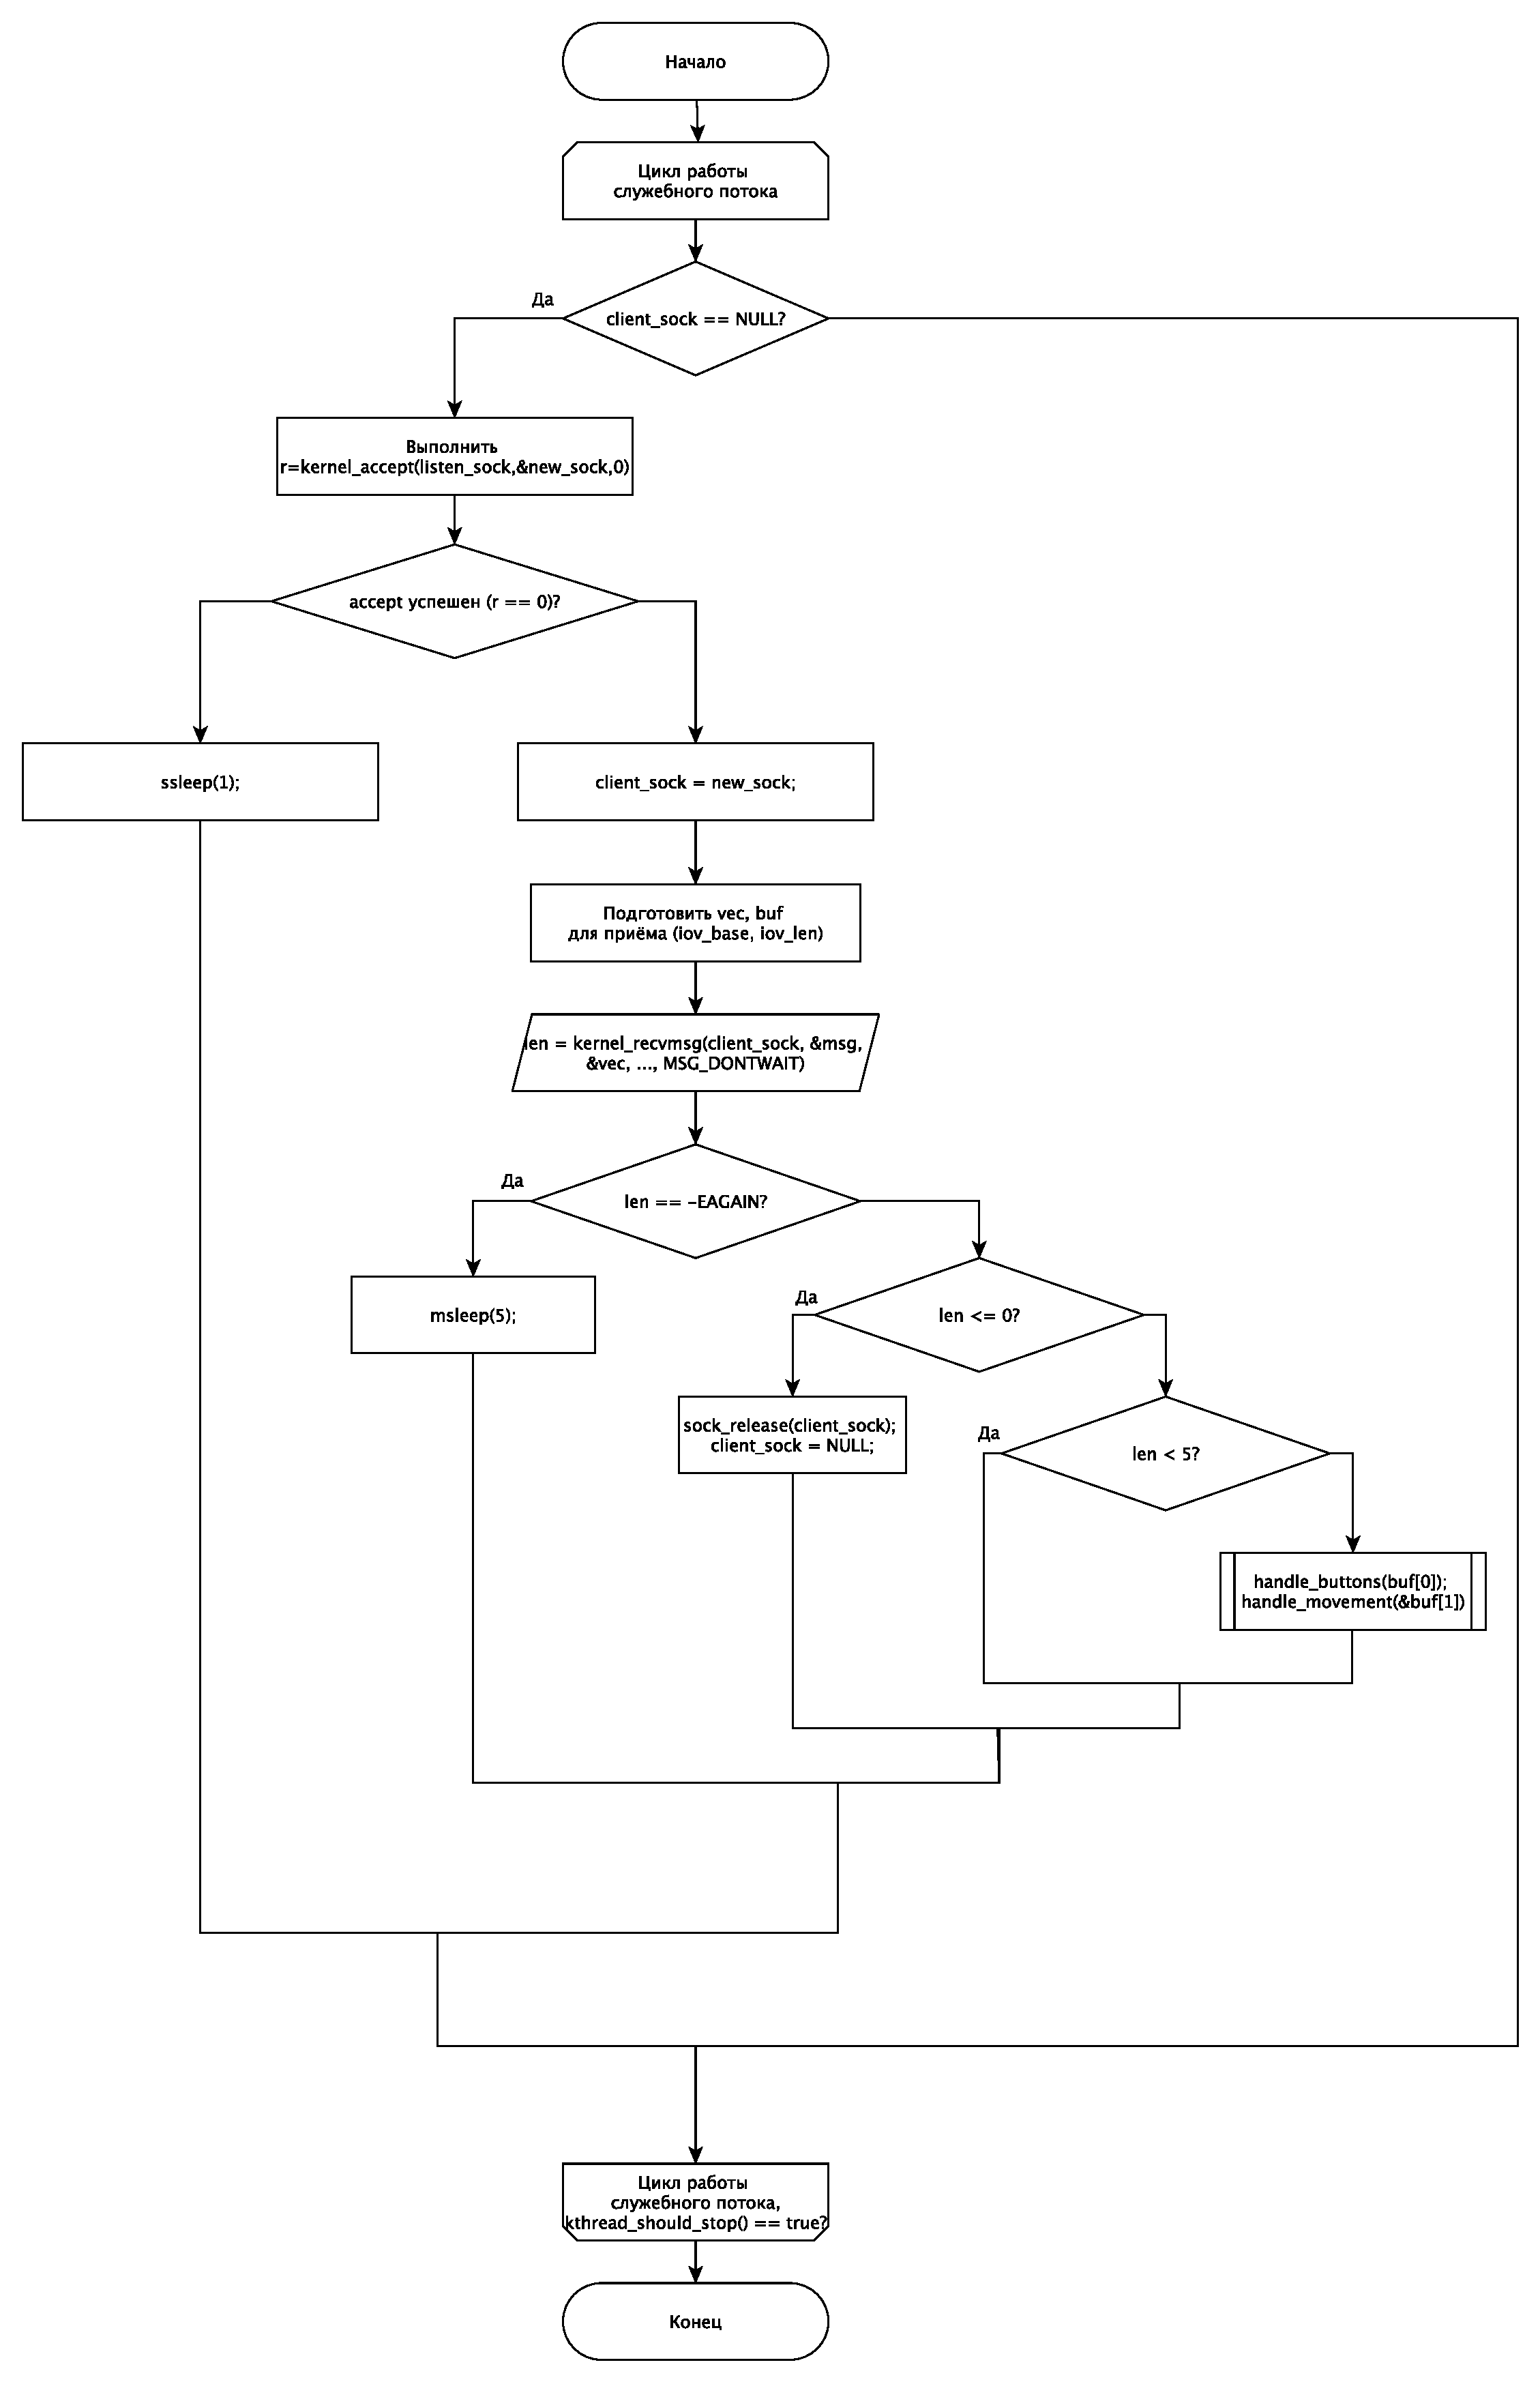
\includegraphics[height=0.7\textheight]{rx-loop.pdf}
	\caption{Схема алгоритма работы служебного потока \texttt{rx\_loop}}
	\label{fig:rx-loop-scheme}
\end{figure}
\clearpage

Обработка состояний кнопок мыши вынесена в отдельную функцию \lstinline|handle_buttons|. Эта функция декодирует битовую маску нажатых кнопок и порождает для каждой активной кнопки последовательность событий нажатия и отпускания с вызовами \lstinline|input_report_key| и \lstinline|input_sync|, формируя короткие клики левой и правой кнопок мыши. Схема алгоритма \lstinline|handle_buttons| приведена на рис.~\ref{fig:handle-buttons-scheme}.

\begin{figure}[h!]
	\centering
	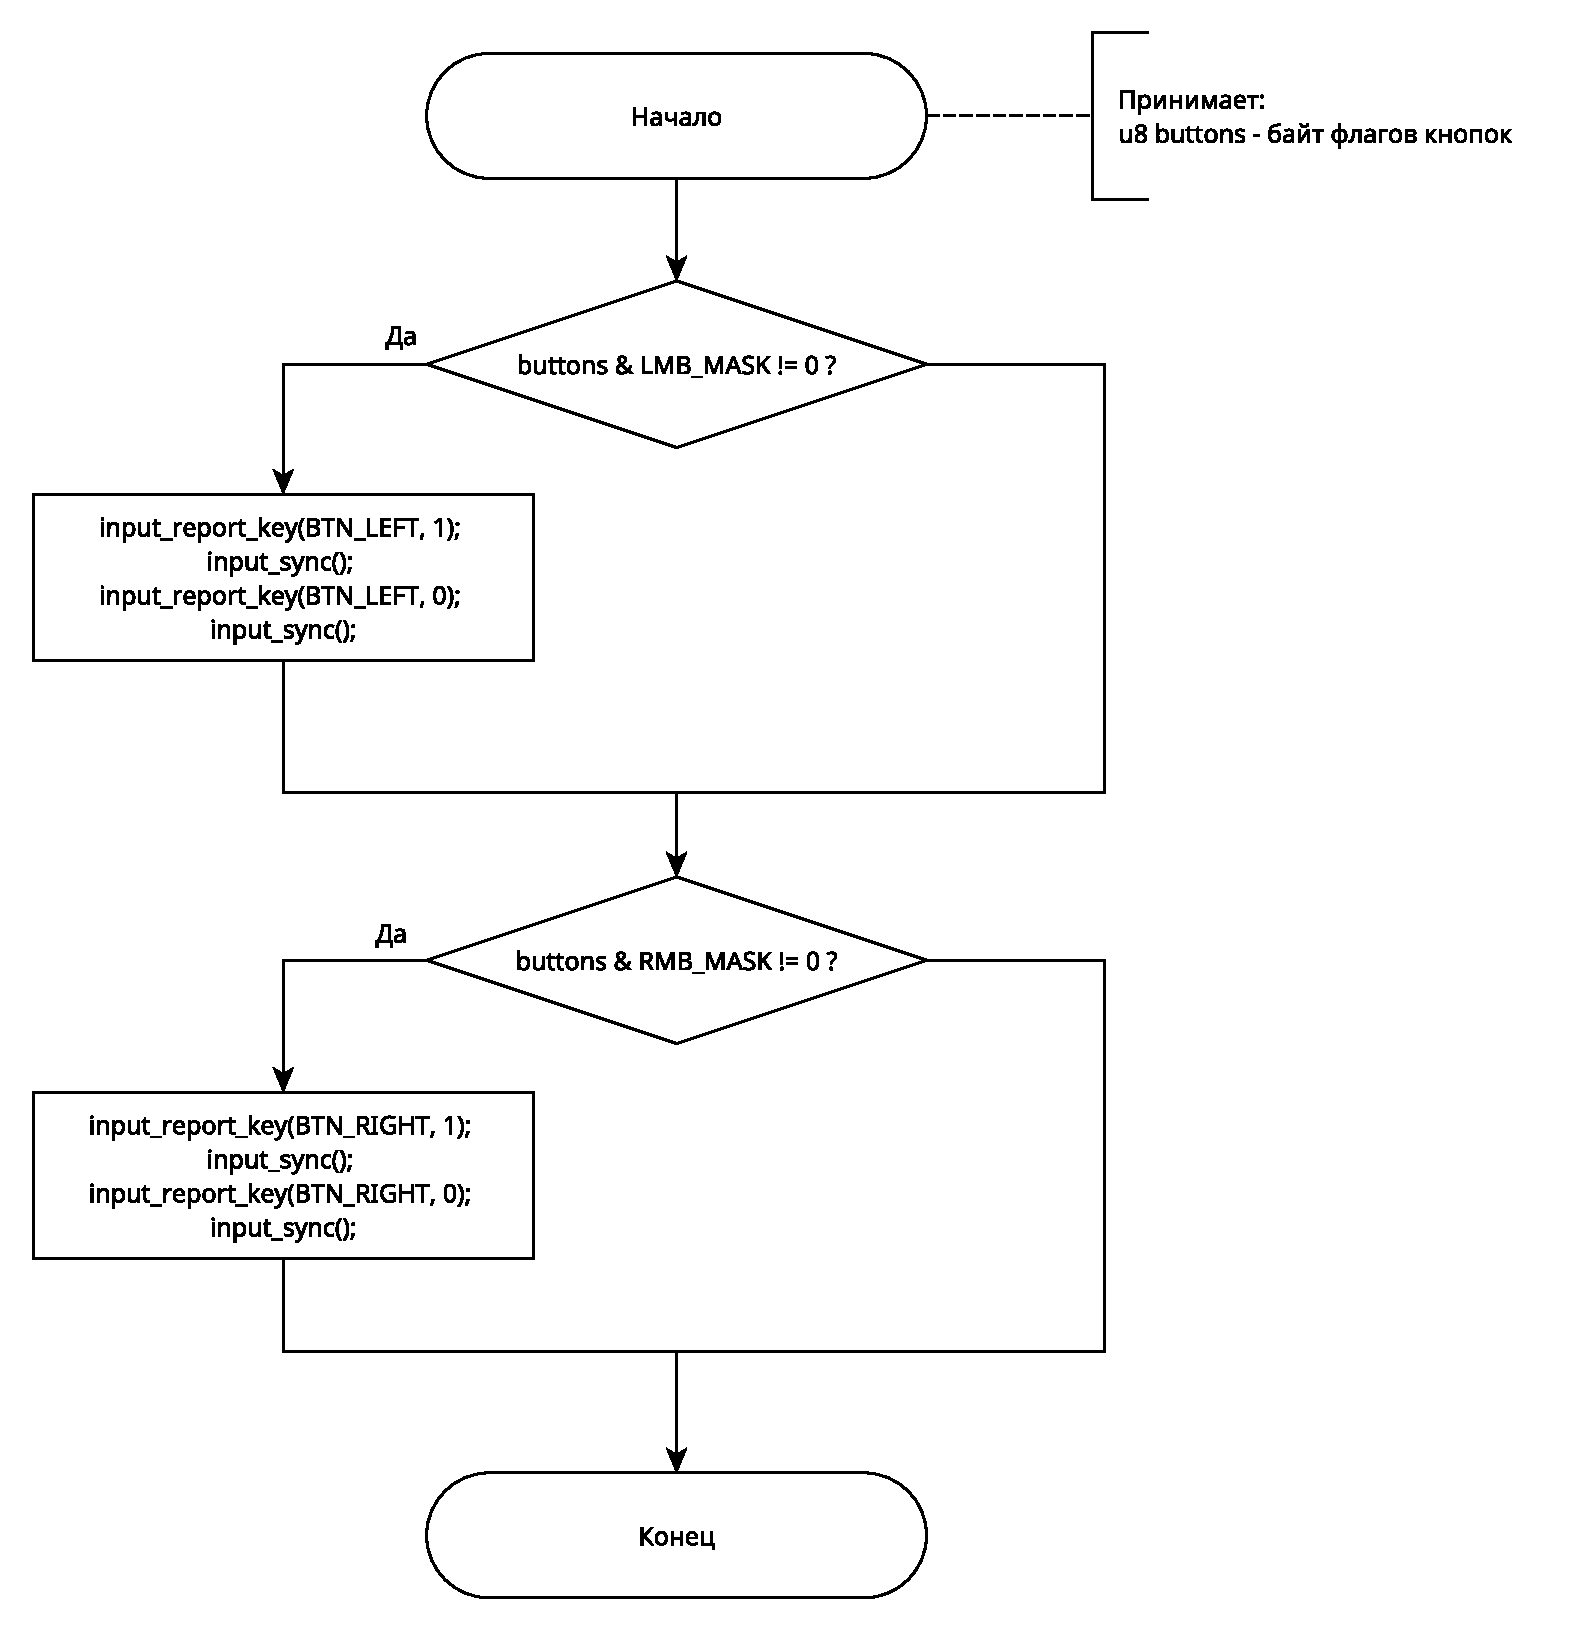
\includegraphics[height=0.7\textheight]{handle_buttons.pdf}
	\caption{Схема алгоритма обработки нажатий кнопок мыши \lstinline|handle_buttons|}
	\label{fig:handle-buttons-scheme}
\end{figure}
\clearpage

Обработка движения курсора реализована в функции \lstinline|handle_movement|. Функция восстанавливает из четырёх байт 16-разрядные смещения по осям, масштабирует их с использованием коэффициента \lstinline|speed_mult| в формате Q16.16 и, в зависимости от значения \lstinline|interp_steps|, либо разбивает движение на несколько мелких шагов с генерацией последовательности событий \lstinline|REL_X| и \lstinline|REL_Y|, либо передаёт смещения единым событием. В обоих случаях каждое изменение сопровождается вызовом \lstinline|input_sync| для фиксации событий подсистемой ввода. Алгоритм функции \lstinline|handle_movement| представлен на рис.~\ref{fig:handle-movement-scheme}.


\begin{figure}[h!]
	\centering
	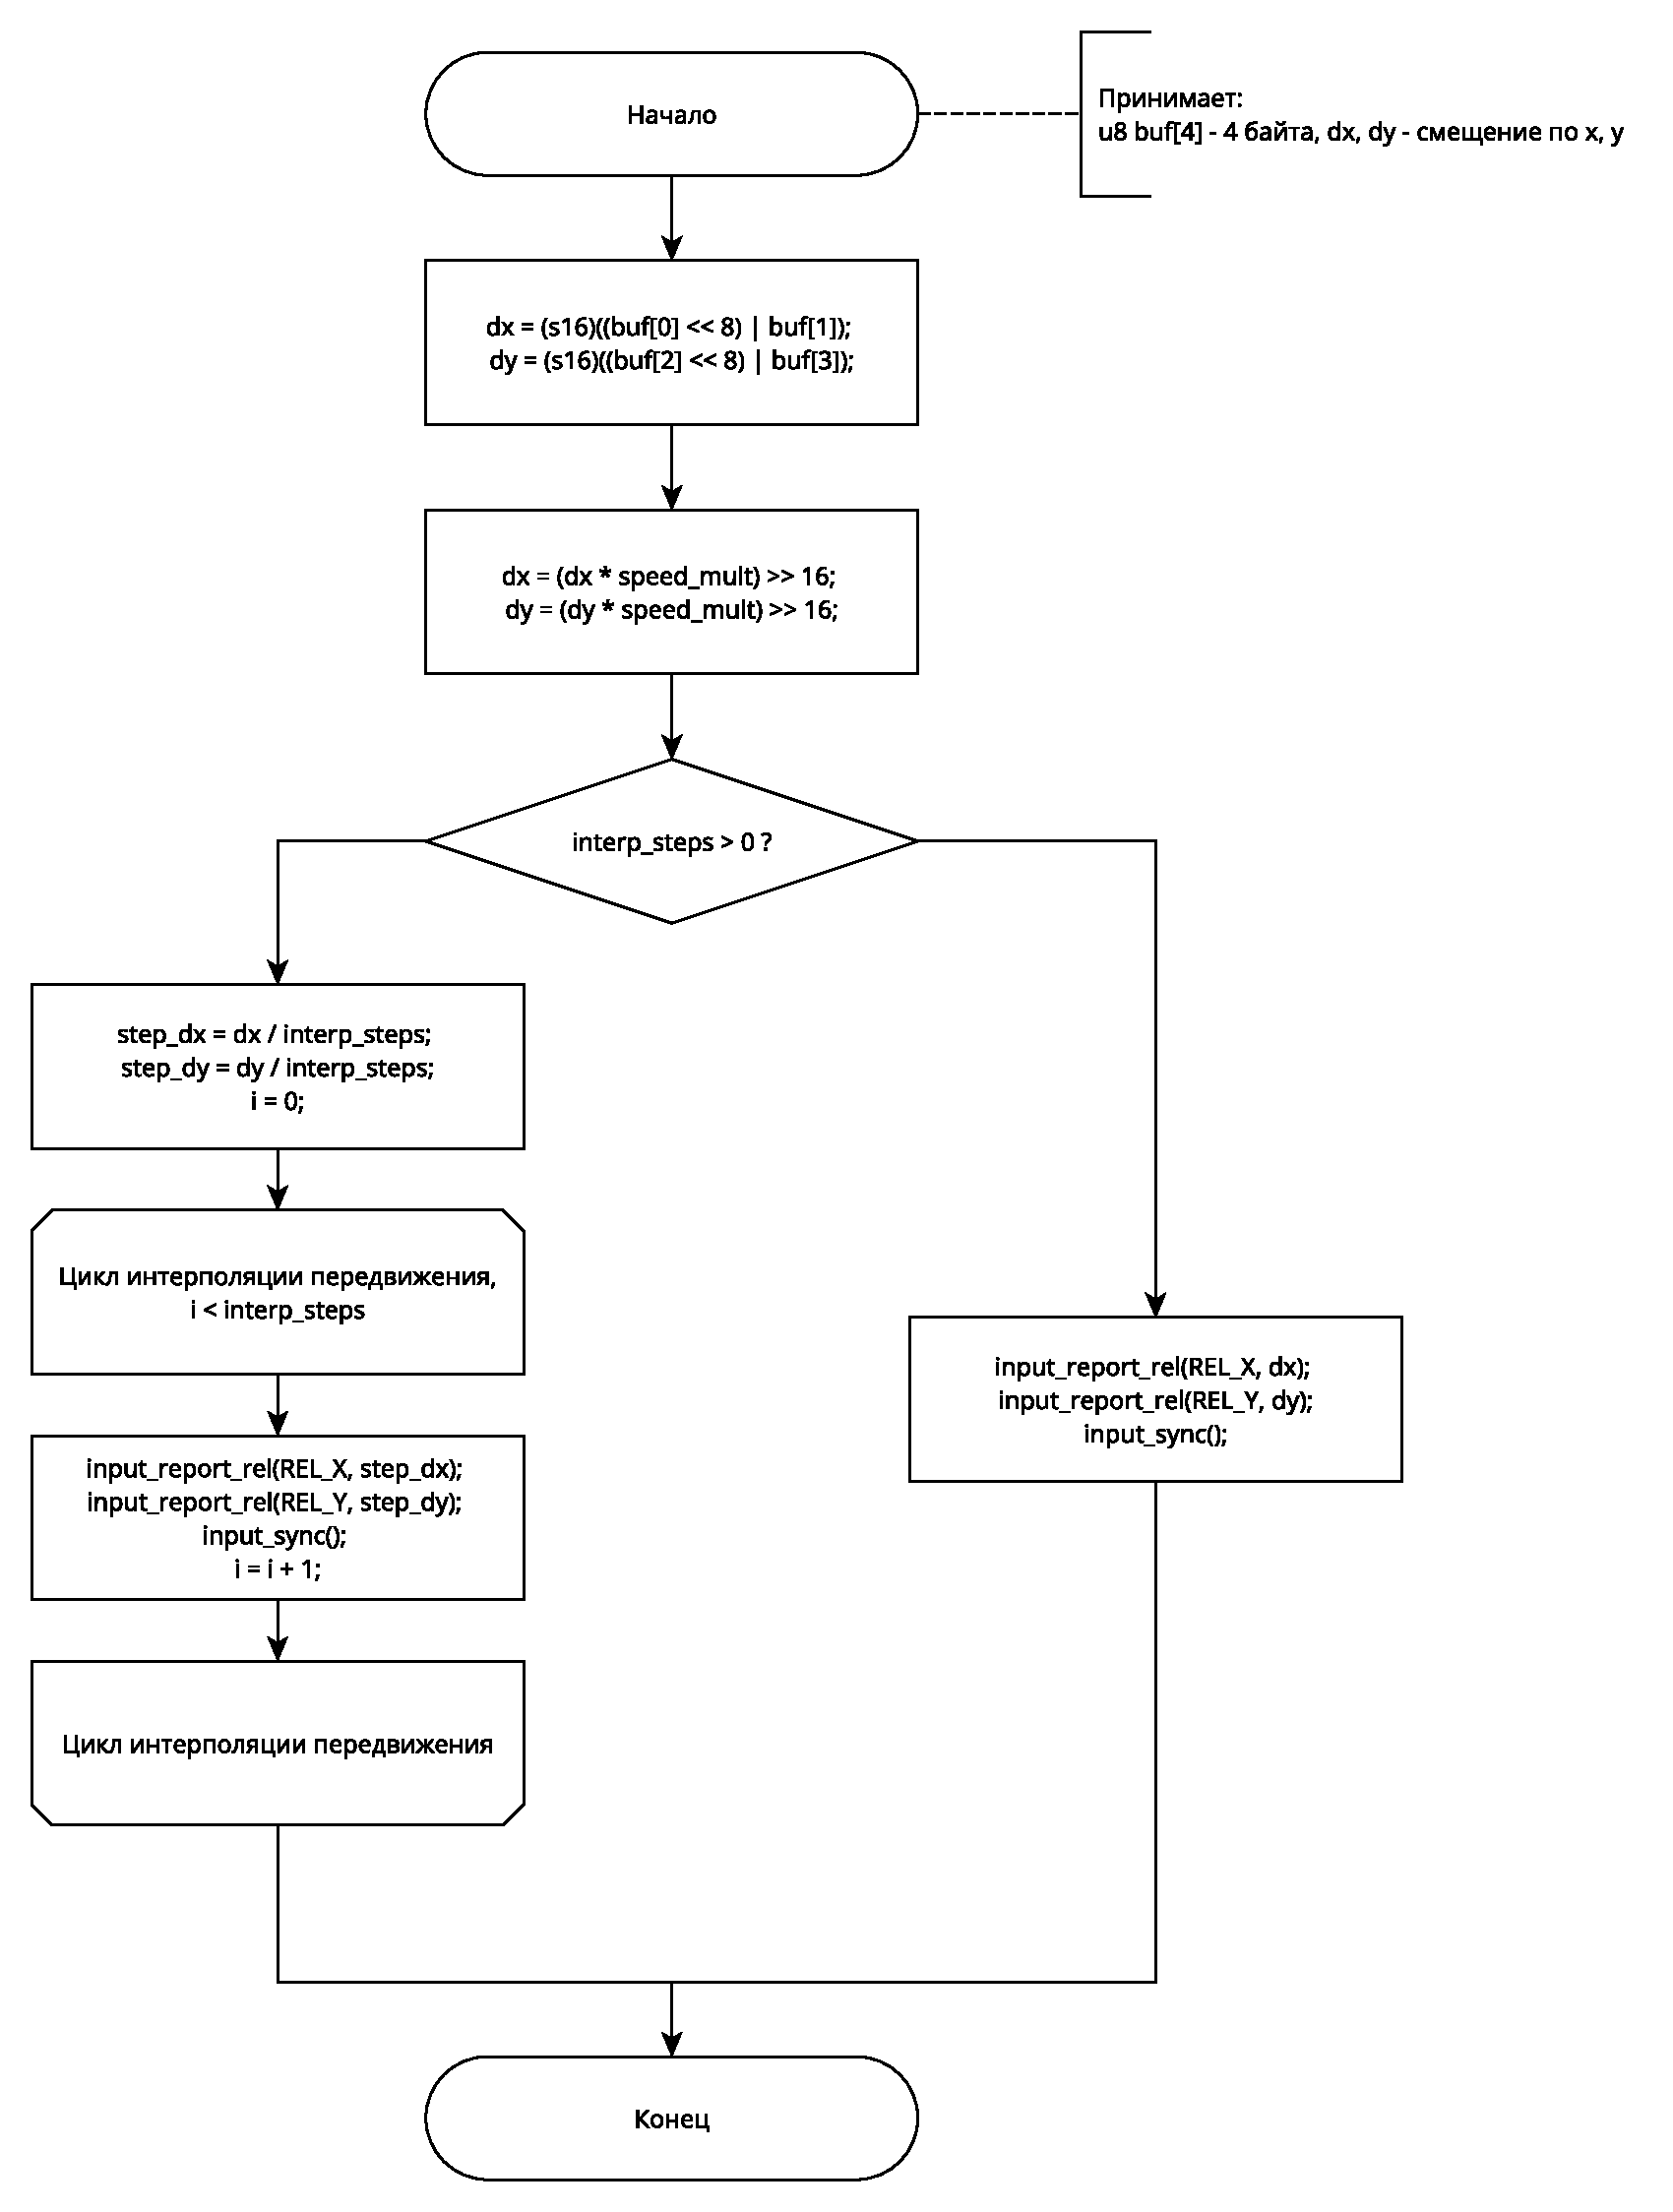
\includegraphics[width=0.7\textwidth]{handle_movement.pdf}
	\caption{Схема алгоритма обработки движения курсора \lstinline|handle_movement|}
	\label{fig:handle-movement-scheme}
\end{figure}
\clearpage

Завершение работы модуля включает остановку служебного потока, закрытие клиентского и серверного RFCOMM-сокетов, снятие виртуального устройства с регистрации и освобождение ресурсов. Последовательность действий функции \lstinline|pm_exit|, зарегистрированной через \lstinline|module_exit|, приведена на рис.~\ref{fig:module-exit-scheme}~\cite{linux-driver-basics,linux-input-docs}.

\begin{figure}[h!]
	\centering
	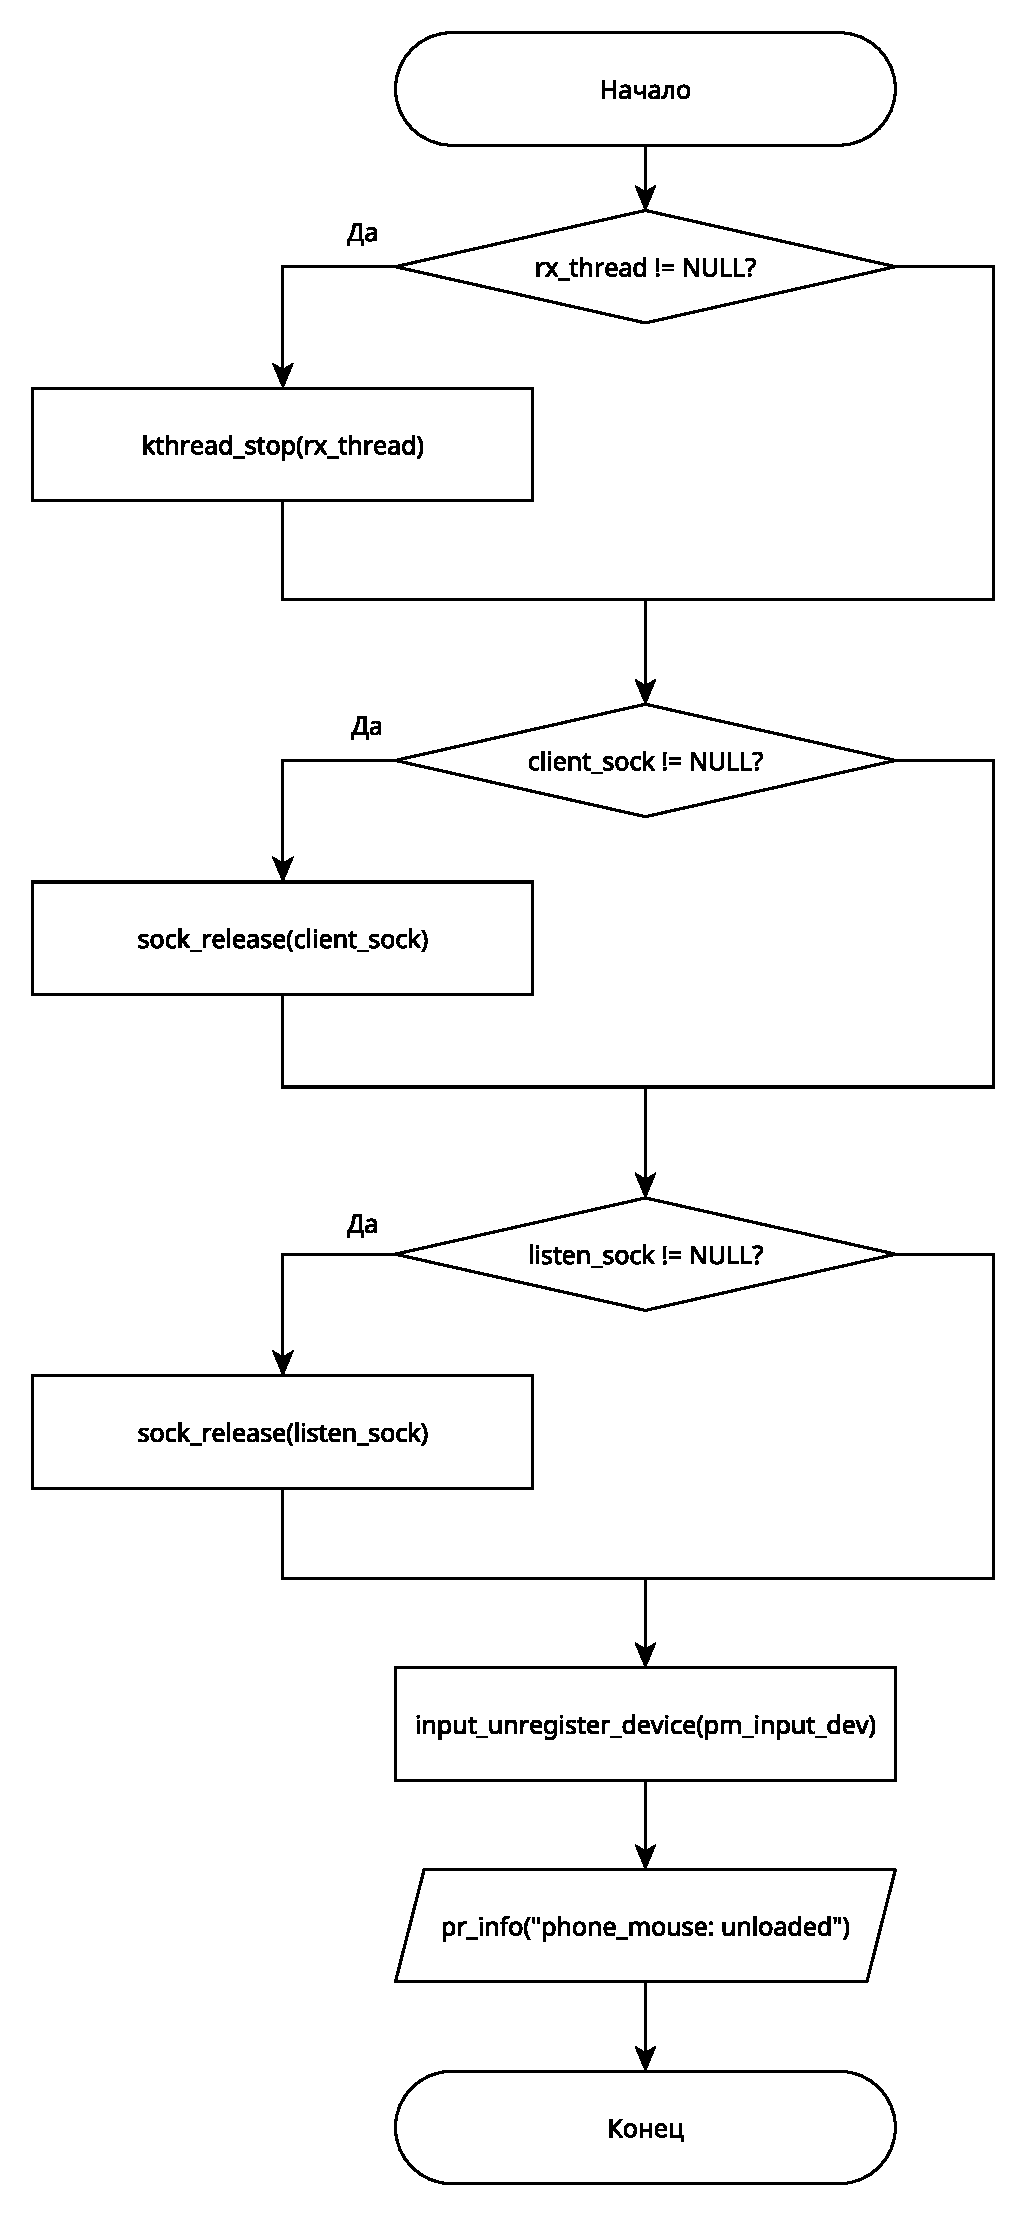
\includegraphics[height=0.7\textheight]{module-exit-scheme.pdf}
	\caption{Схема алгоритма завершения работы модуля ядра \texttt{phone\_mouse\_bt}}
	\label{fig:module-exit-scheme}
\end{figure}
\clearpage

\subsection{Последовательность работы мобильного приложения}

Мобильное приложение реализовано в виде т. н. "Android-активности" (Activity), которая инициализирует пользовательский интерфейс, запускает фоновый поток отправки накопленных смещений курсора, устанавливает Bluetooth-соединение с рабочей станцией и обрабатывает события сенсорного экрана и нажатия кнопок мыши~\cite{android-bt-connect,BluetoothSocket-doc}. Общая последовательность работы основной активности \lstinline|MainActivity| представлена на рис.~\ref{fig:app-main-activity}: при создании активности выполняется настройка интерфейса, запуск фонового потока отправки движения, восстановление сохранённого MAC-адреса, установка обработчиков для поля ввода MAC-адреса, кнопок мыши и области touchpad, а также, при наличии сохранённого адреса, инициируется подключение к рабочей станции.

\begin{figure}[h!]
	\centering
	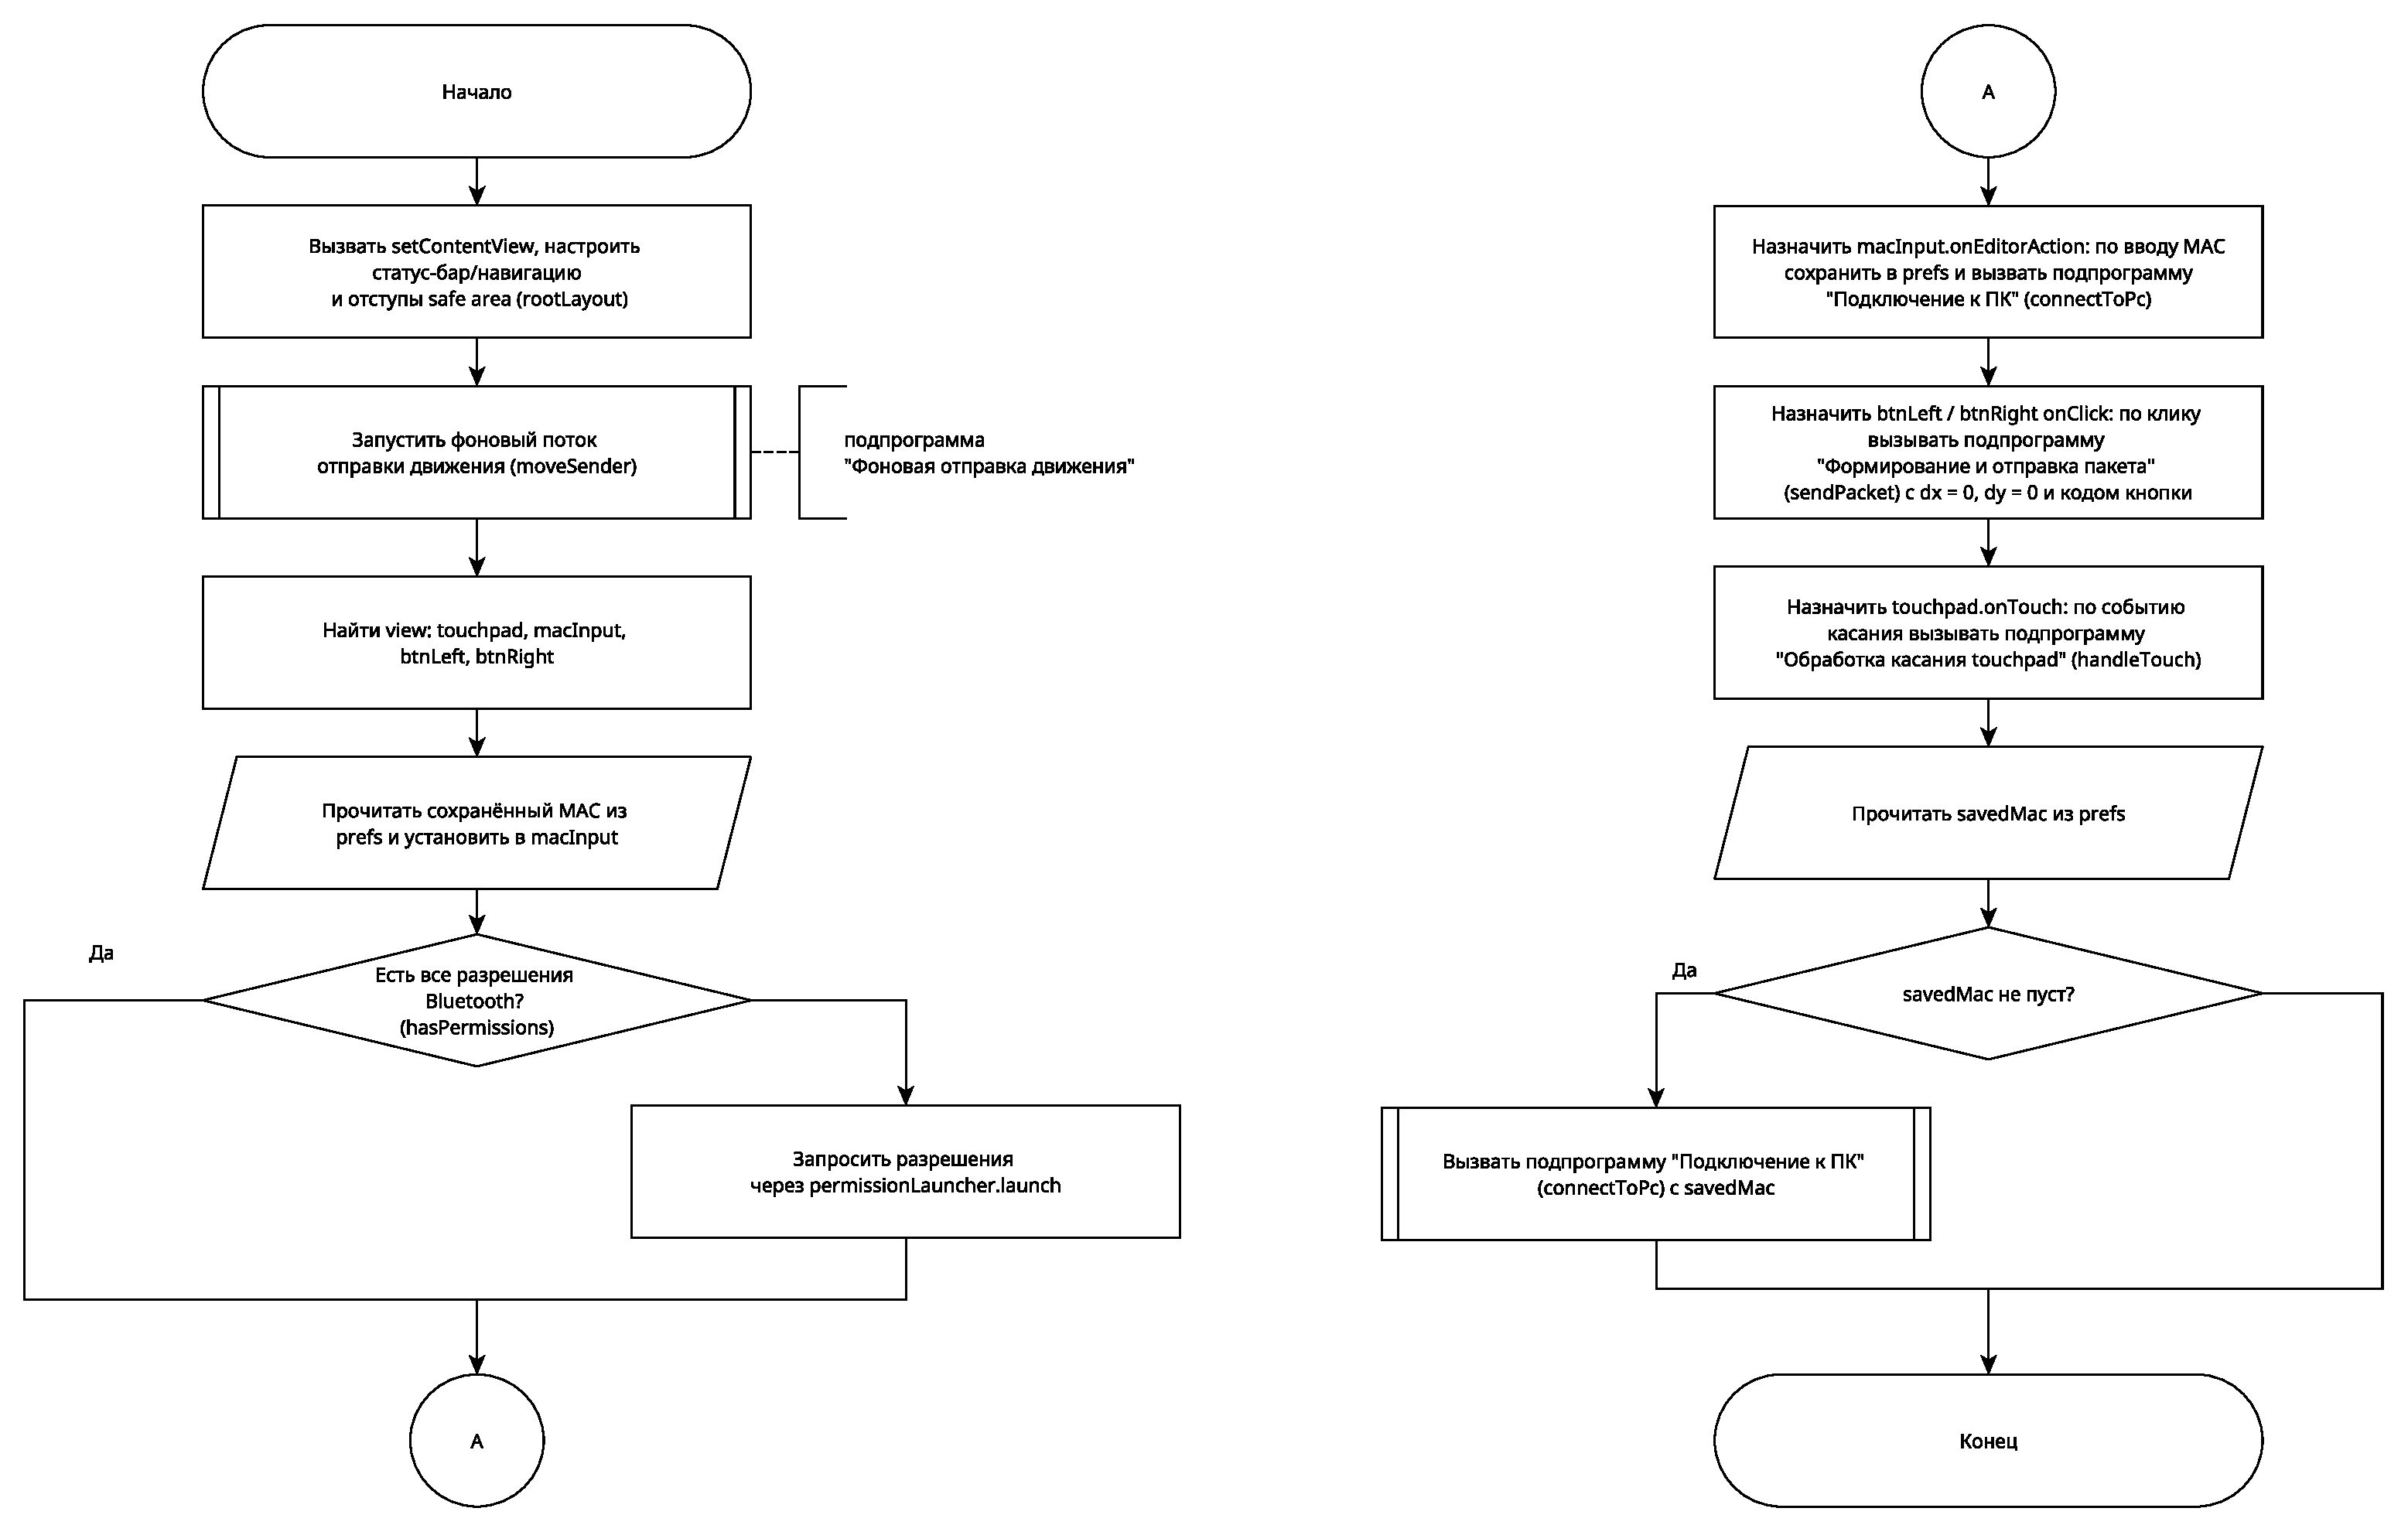
\includegraphics[width=0.9\textwidth]{AppMainActivity.pdf}
	\caption{Схема алгоритма работы основной активности мобильного приложения}
	\label{fig:app-main-activity}
\end{figure}
\clearpage

Отправка накопленных смещений курсора реализована в отдельном потоке, который с фиксированным интервалом времени считывает значения переменных \lstinline|pendingDx| и \lstinline|pendingDy|, обнуляет накопленные значения и, при ненулевых смещениях, формирует пакет данных о смещении курсора, которая отправляется на устройство-обработчик с помощью вызова \lstinline|sendPacket|. Алгоритм работы данного потока показан на рис.~\ref{fig:sendpacket-thread}.

\begin{figure}[h!]
	\centering
	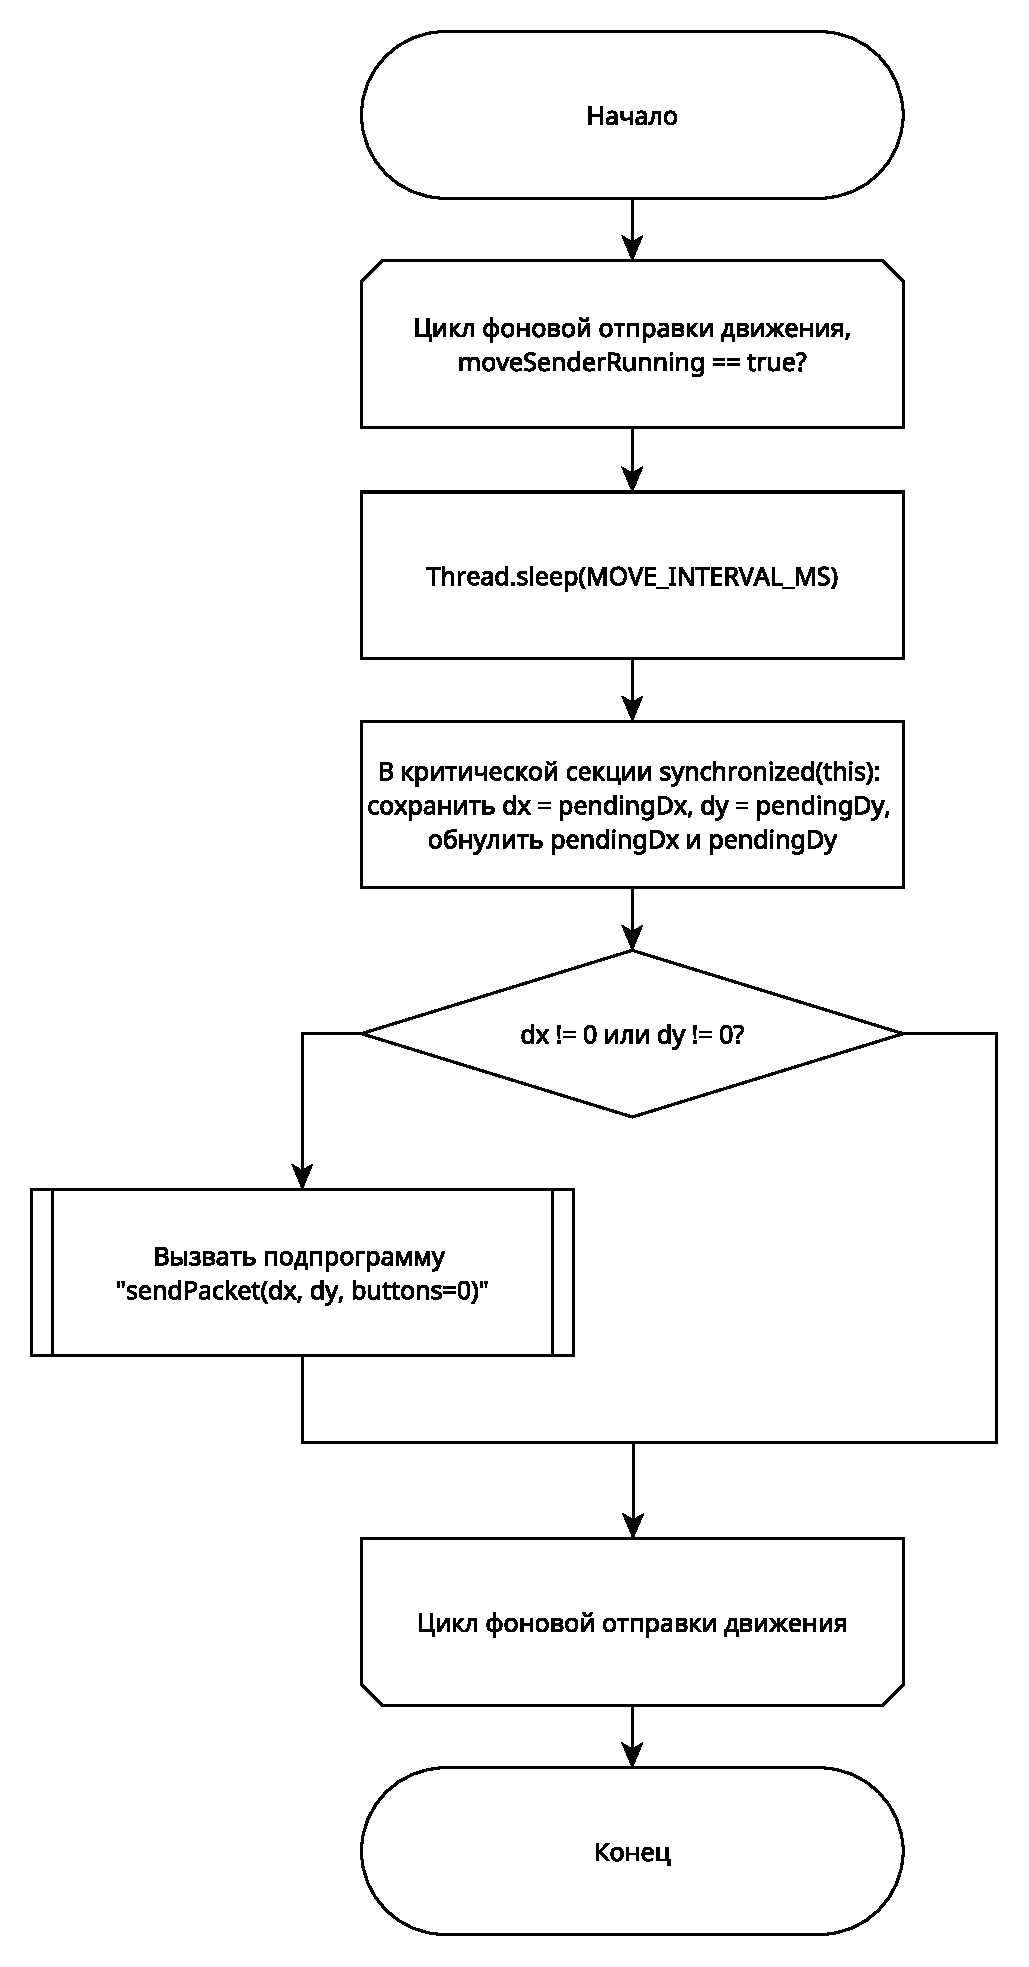
\includegraphics[height=0.7\textheight]{SendPacketThread.pdf}
	\caption{Схема алгоритма фонового потока отправки накопленных смещений}
	\label{fig:sendpacket-thread}
\end{figure}
\clearpage

Функция \lstinline|sendPacket| формирует бинарное сообщения протокола из смещений по осям и битовой маски кнопок мыши, проверяет наличие открытого выходного потока, упаковывает значения в массив из пяти байт и выполняет запись массива в \lstinline|OutputStream|, игнорируя исключения ввода-вывода. Последовательность действий функции \lstinline|sendPacket| представлена на рис.~\ref{fig:sendpacket-func}.

\begin{figure}[h!]
	\centering
	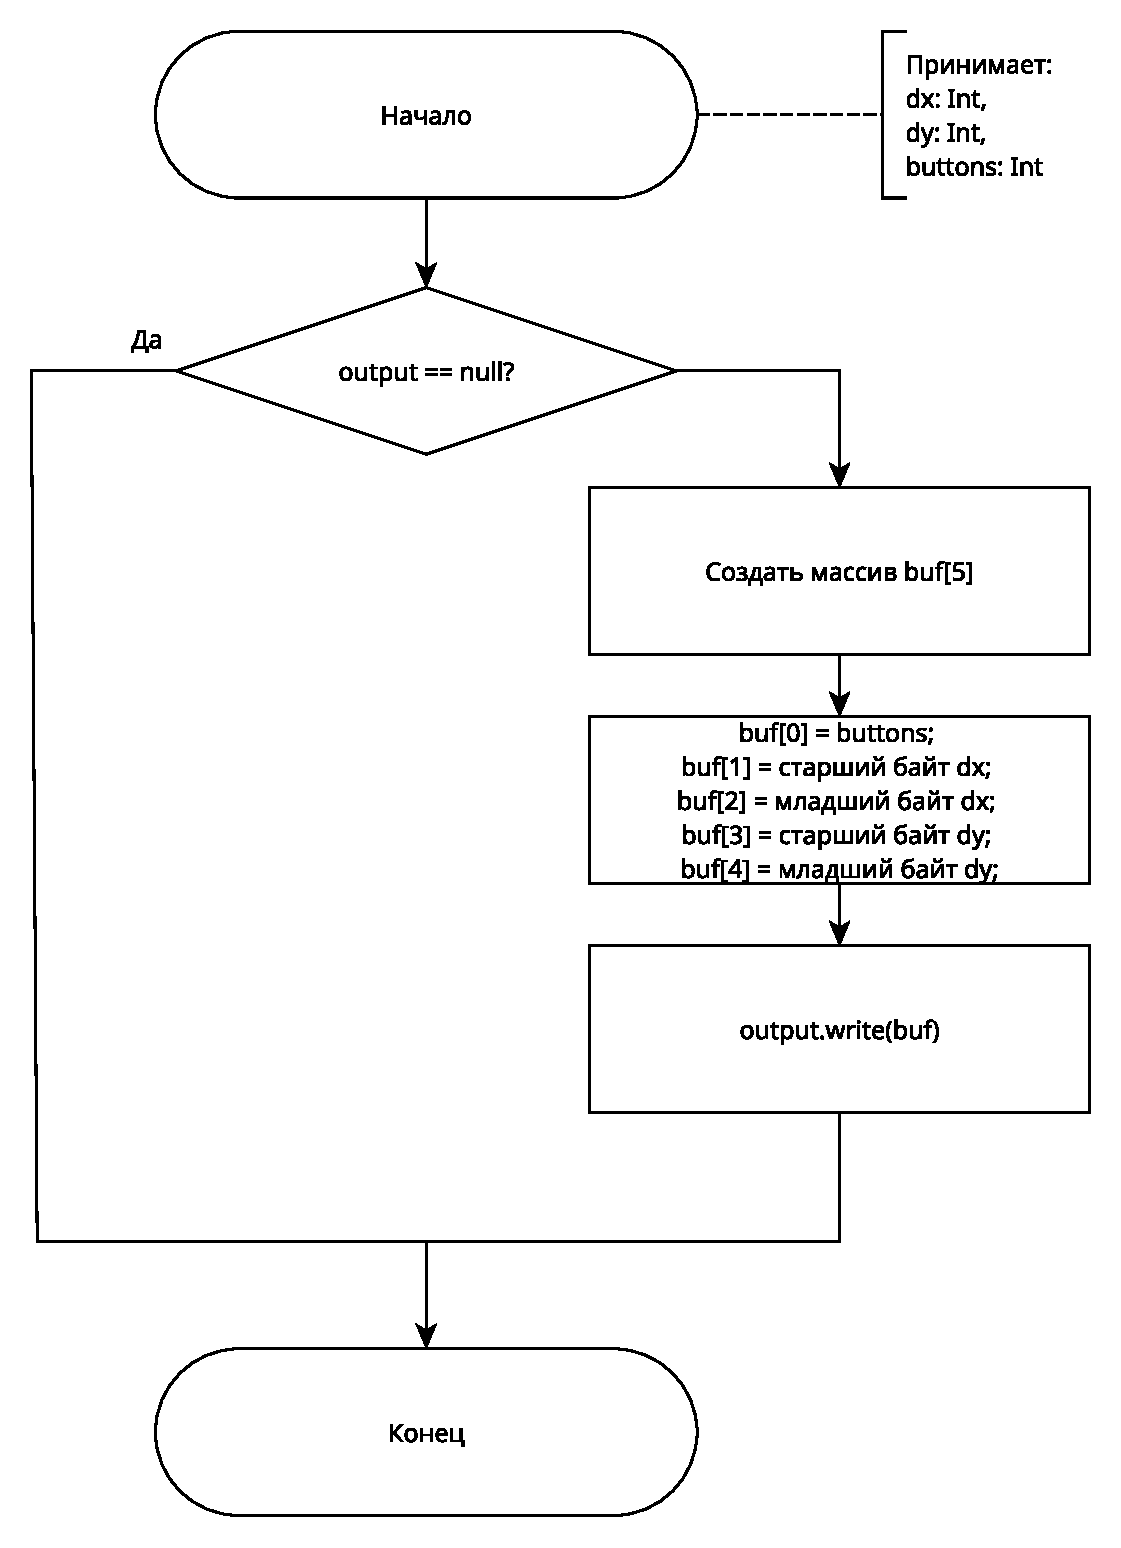
\includegraphics[width=0.8\textwidth]{SendPacket.pdf}
	\caption{Схема алгоритма формирования и отправки пакета команд \lstinline|sendPacket|}
	\label{fig:sendpacket-func}
\end{figure}
\clearpage

Установление соединения с целевым устройством выполняется функцией \lstinline|connectToPc|, которая проверяет корректность введённого MAC-адреса, получает адаптер Bluetooth, инициирует фоновый поток подключения, создаёт RFCOMM-сокет к указанному каналу, выполняет соединение и сохраняет \lstinline|BluetoothSocket| и поток вывода. В случае успеха и при ошибках пользователю отображаются диагностические сообщения. Общий алгоритм функции \lstinline|connectToPc| показан на рис.~\ref{fig:connect-to-pc}, а внутренний поток подключения, использующий вызовы сокета и обработку исключений, представлен отдельно на рис.~\ref{fig:connect-to-pc-thread}.

\begin{figure}[h!]
	\centering
	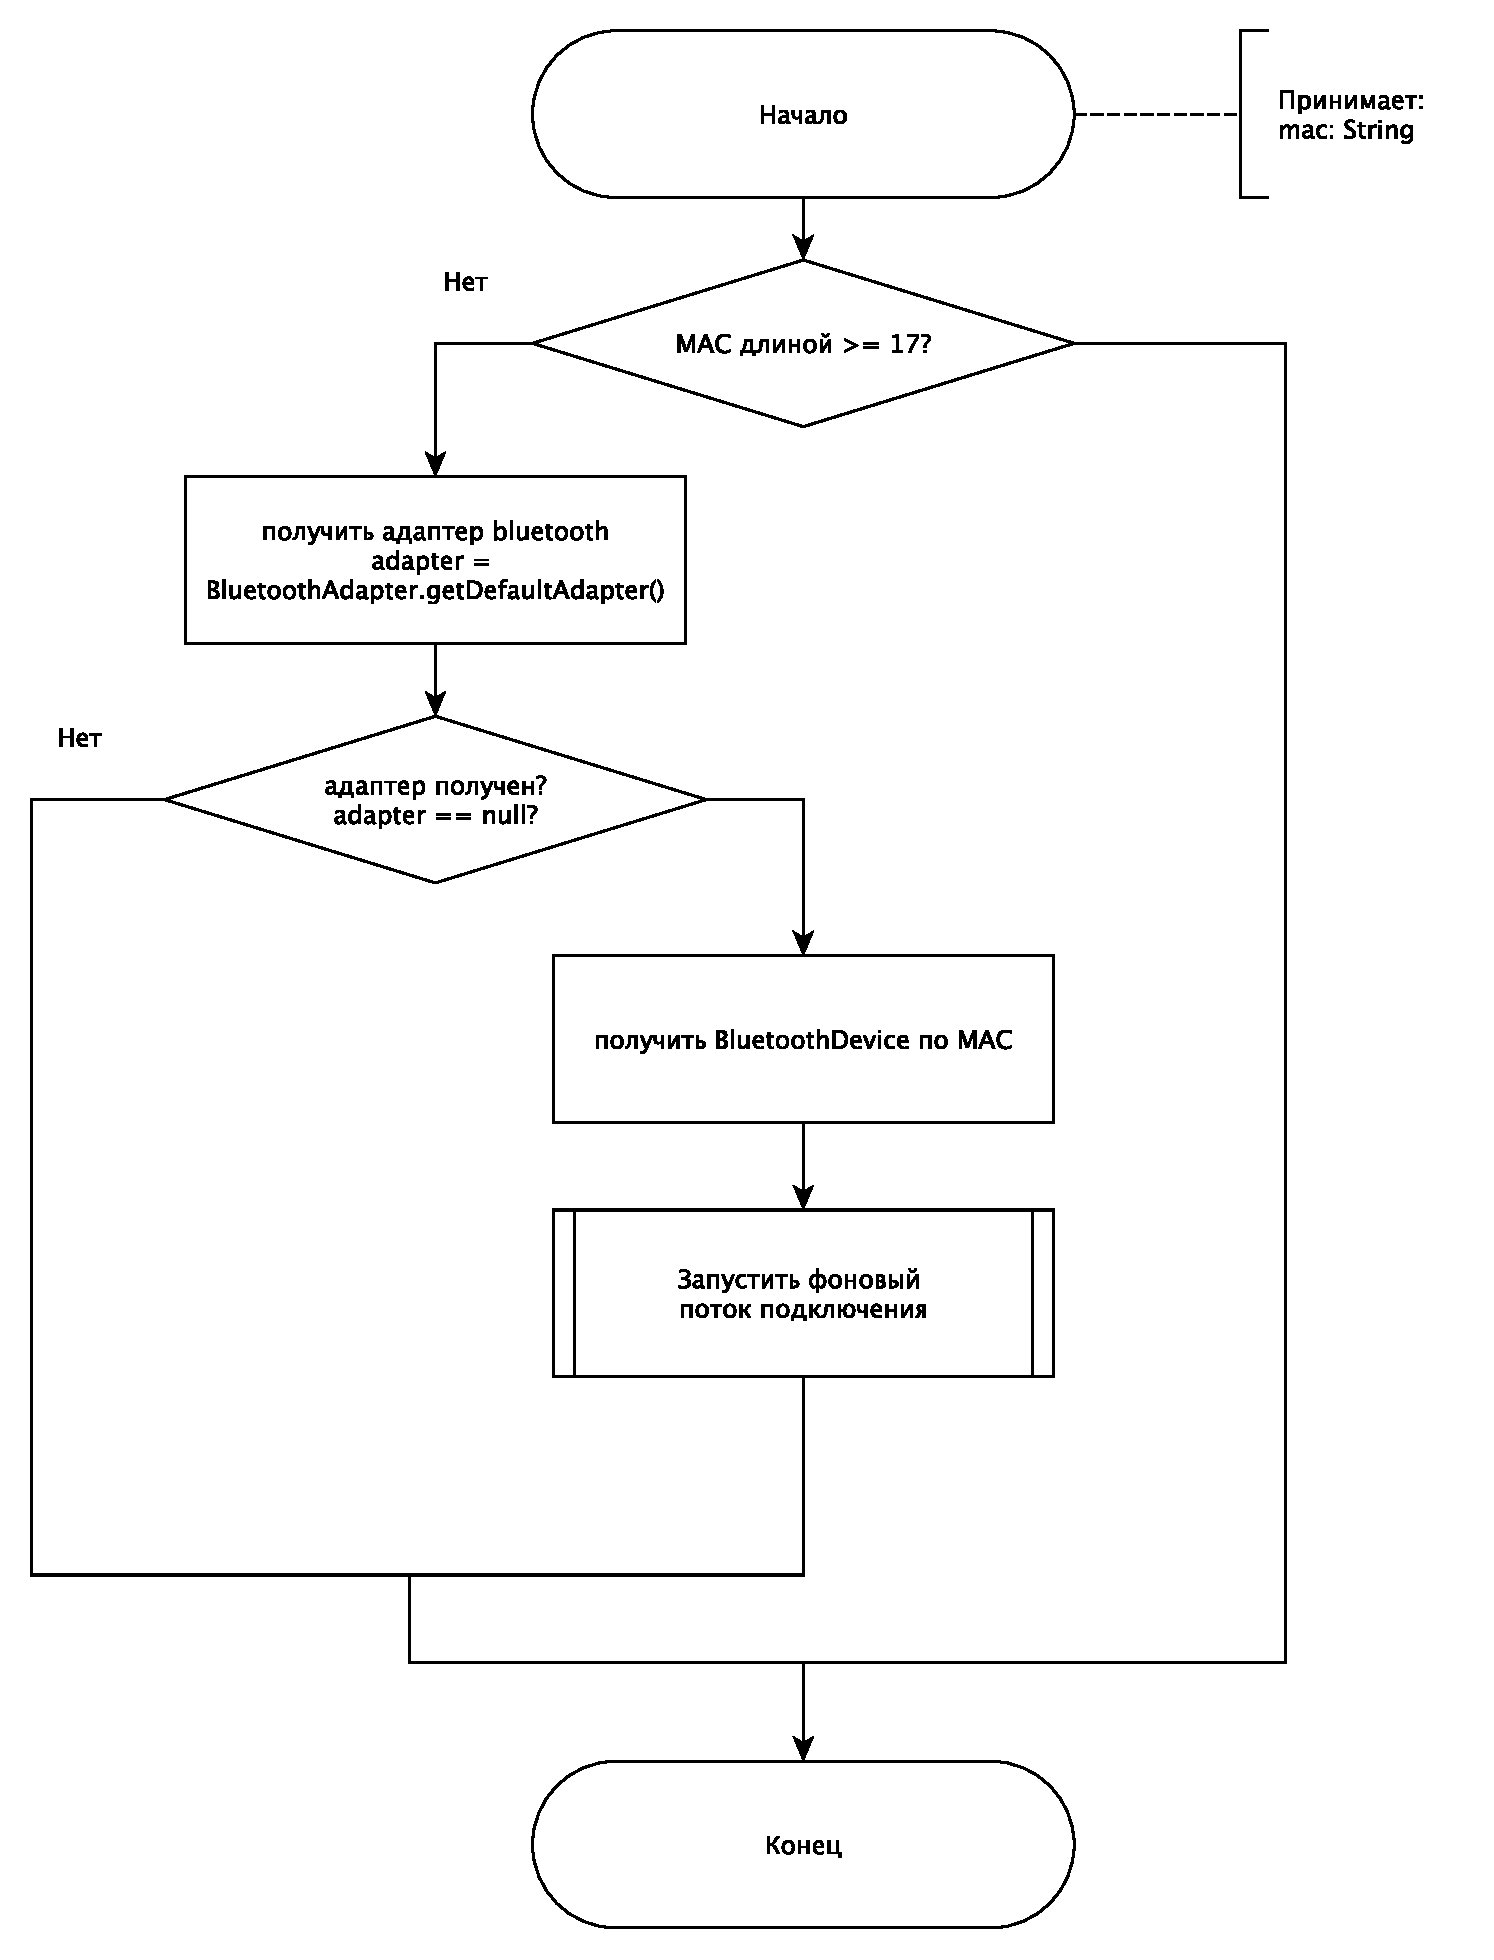
\includegraphics[height=0.7\textheight]{ConnectToPc.pdf}
	\caption{Схема алгоритма функции подключения к рабочей станции \lstinline|connectToPc|}
	\label{fig:connect-to-pc}
\end{figure}
\clearpage

\begin{figure}[h!]
	\centering
	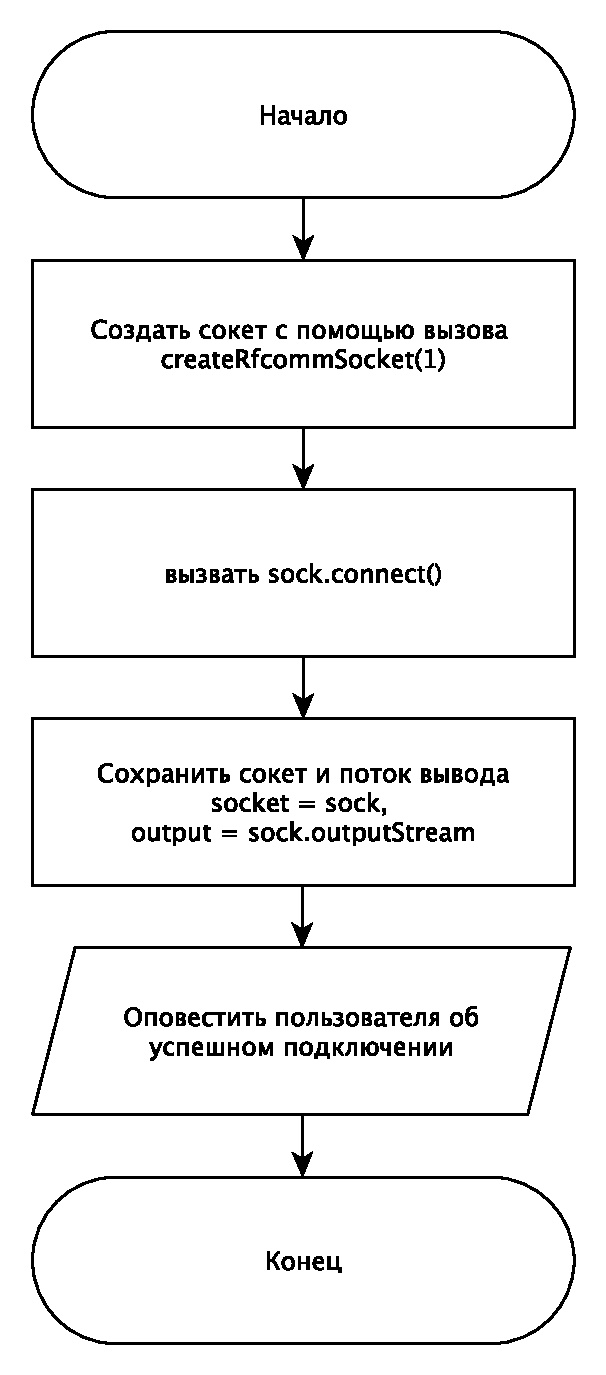
\includegraphics[height=0.9\textheight]{ConnectToPcInnerThread.pdf}
	\caption{Схема алгоритма внутреннего потока установления RFCOMM-соединения}
	\label{fig:connect-to-pc-thread}
\end{figure}
\clearpage


Обработка движения пальца по сенсорной области реализована в функции \lstinline|handleTouch|, которая по событию \lstinline|ACTION_DOWN| запоминает исходные координаты и сбрасывает флаг первого движения, а по событиям \lstinline|ACTION_MOVE| вычисляет относительные смещения по осям, обновляет координаты последнего касания и в критической секции увеличивает накопленные значения \lstinline|pendingDx| и \lstinline|pendingDy|. Эта логика отражена на рис.~\ref{fig:handle-touch}. Накопленные таким образом смещения затем периодически считываются фоновым потоком, изображённым на рис.~\ref{fig:sendpacket-thread}, и передаются в драйвер.

\begin{figure}[h!]
	\centering
	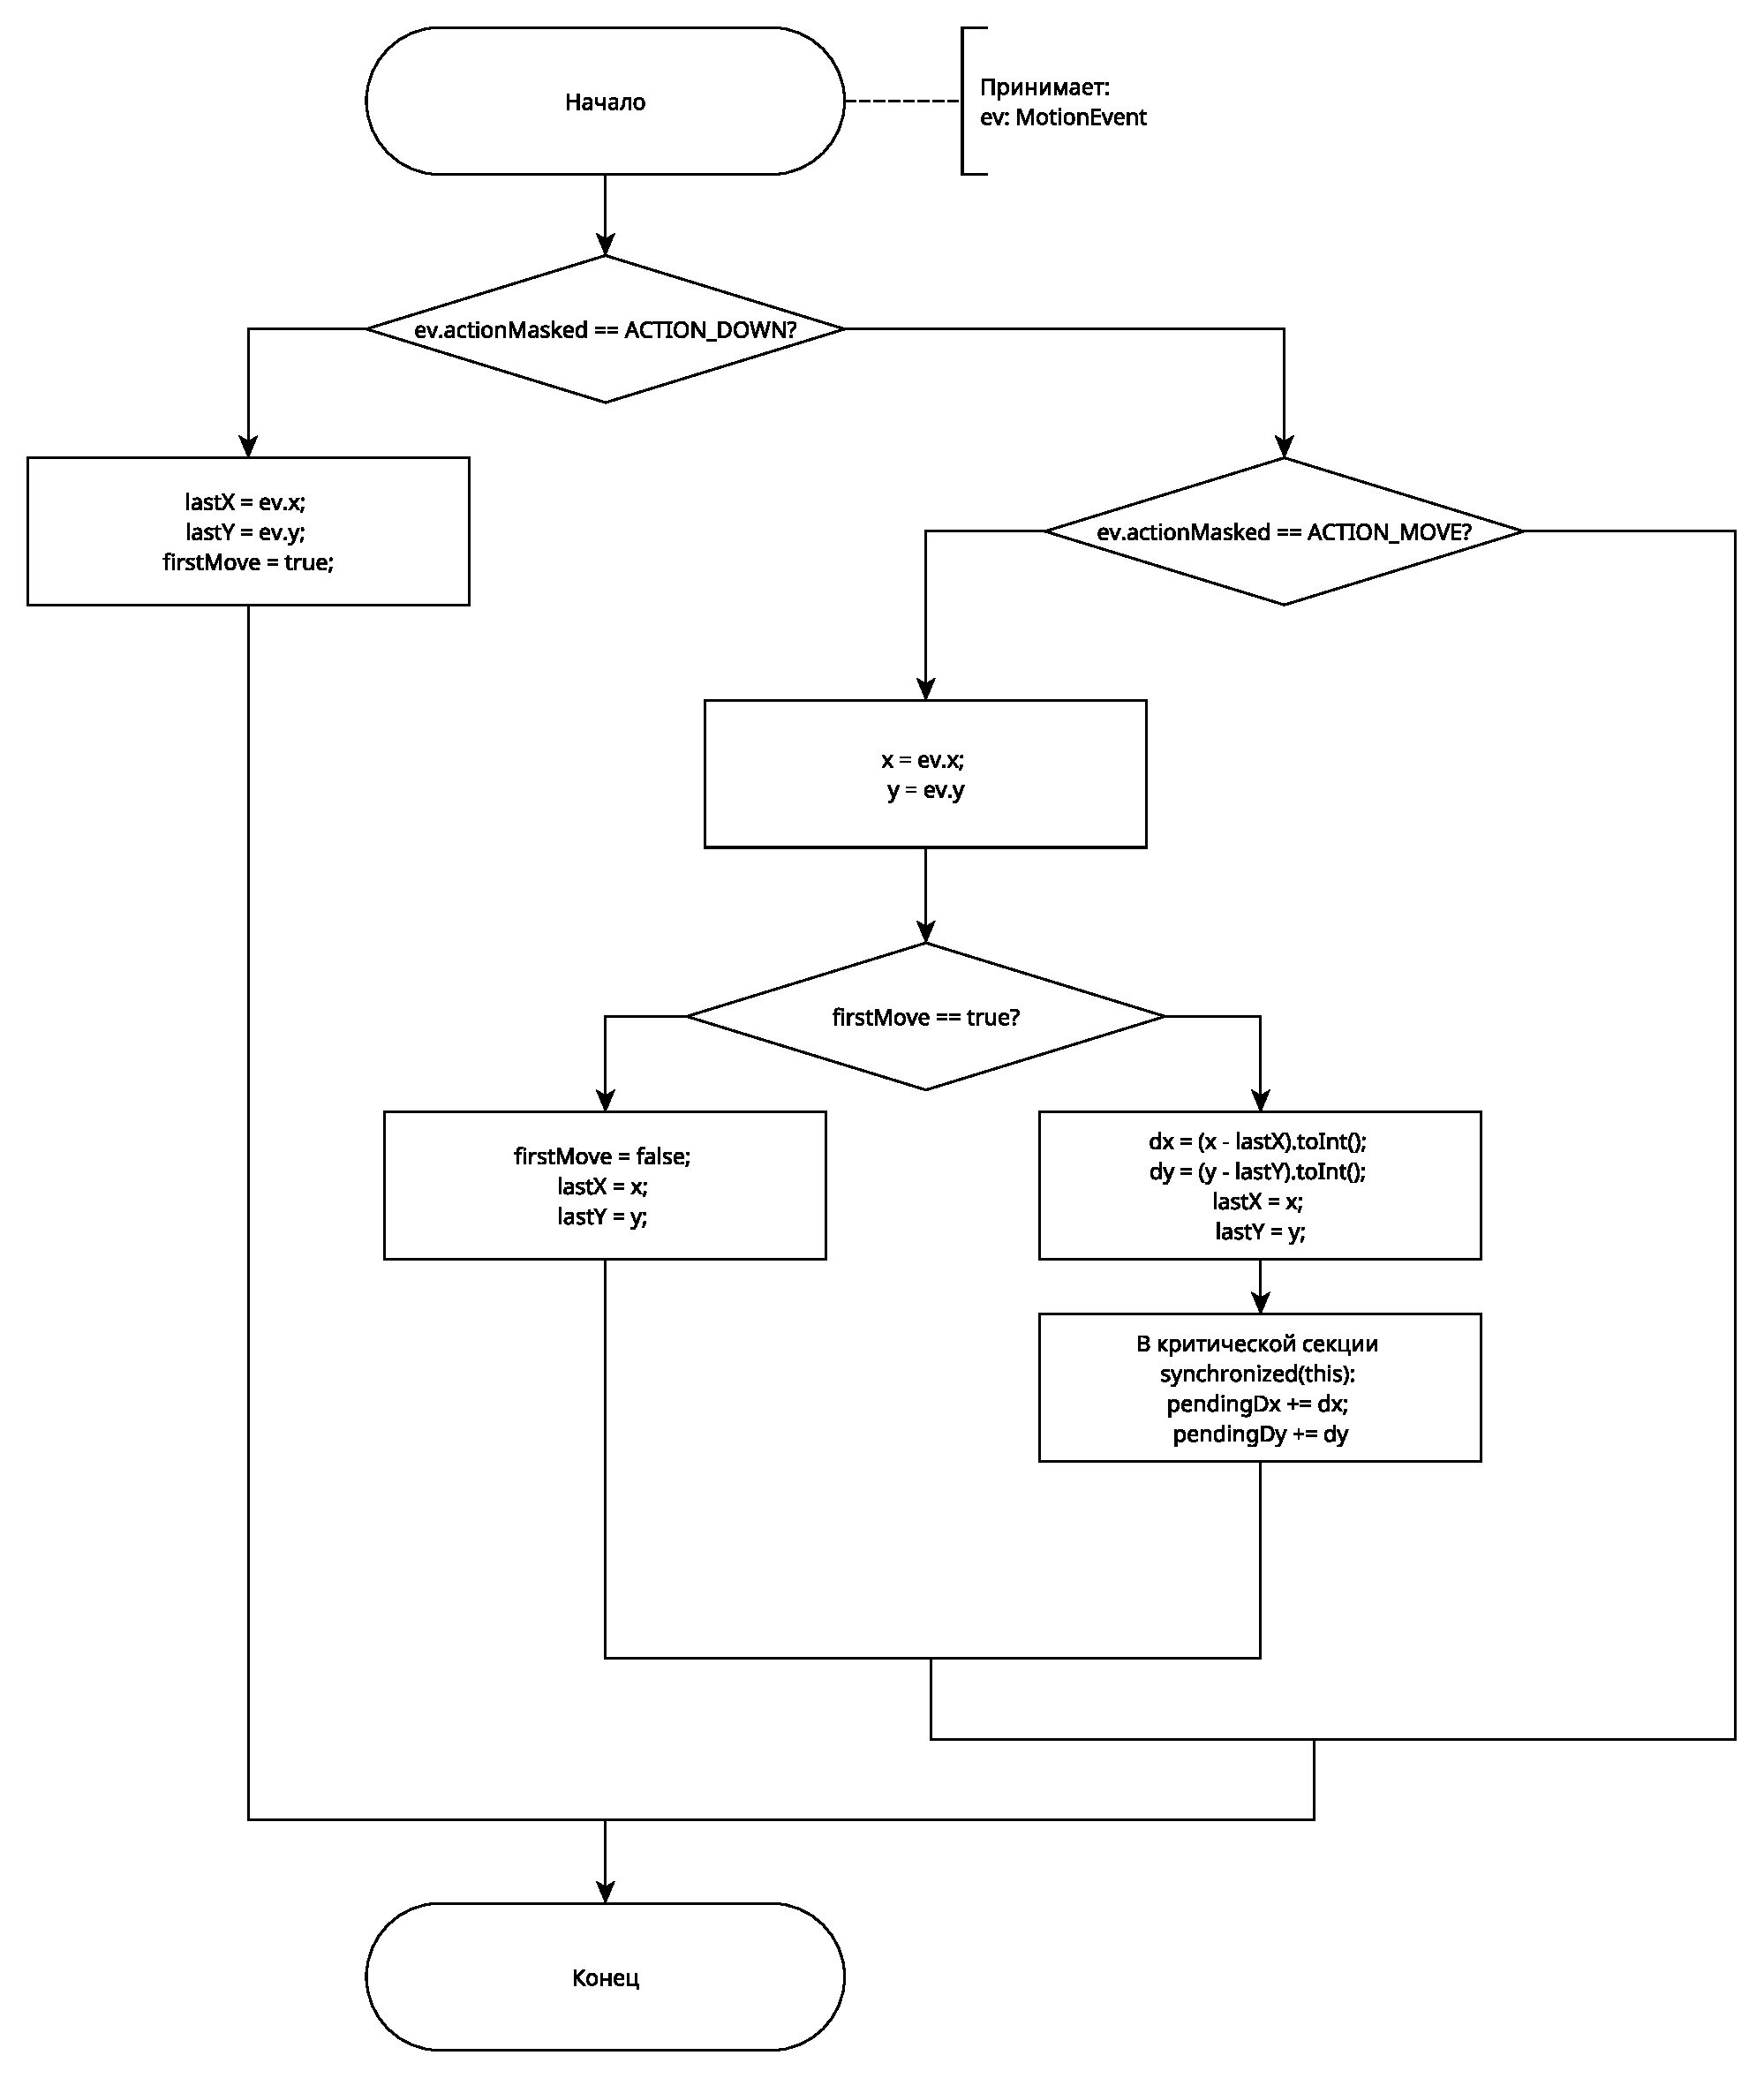
\includegraphics[width=0.9\textwidth]{HandleTouch.pdf}
	\caption{Схема алгоритма обработки касаний на области touchpad \lstinline|handleTouch|}
	\label{fig:handle-touch}
\end{figure}
\clearpage
